% Mechanism diagram for Paper B. TikZ standalone; one accent colour (orange) plus black and gray.
% Build: tectonic fig_bidirectional.tex --outdir <dir>, then copy the PDF to papers/spectral/figs/.
\documentclass[tikz,border=2pt]{standalone}
\usepackage[T1]{fontenc}
\usepackage{helvet}
\renewcommand{\familydefault}{\sfdefault}
\usetikzlibrary{arrows.meta}
\hyphenpenalty=10000 \exhyphenpenalty=10000
\definecolor{acc}{HTML}{eb6834}
\definecolor{wire}{HTML}{6b6b6b}
\tikzset{
  every node/.style={font=\fontsize{8}{9.5}\selectfont, text=black},
  wire/.style={draw=wire, line width=0.5pt},
  cell/.style={draw=wire, fill=white, line width=0.5pt, minimum size=0.2cm, inner sep=0pt},
  unk/.style={draw=wire, fill=white, line width=0.5pt, minimum size=0.3cm, inner sep=0pt, text=wire, font=\fontsize{8}{9}\selectfont\bfseries},
  bad/.style={draw=black, fill=acc, line width=0.5pt, minimum size=0.28cm, inner sep=0pt},
  band/.style={fill=acc!13, draw=none},
  drv/.style={-{Stealth[length=1.7mm]}, line width=0.8pt, black},
  drvb/.style={-{Stealth[length=1.7mm]}, line width=0.8pt, black, dash pattern=on 2pt off 1.5pt},
  flag/.style={fill=acc, draw=black, line width=0.4pt},
  quiet/.style={fill=gray!45, draw=none},
}
% 5x5 crossbar, pitch 0.62 cm. Column c at x=X(c), row r at y=Y(r).
\newcommand{\X}[1]{(0.31+0.62*(#1-1))}
\newcommand{\Y}[1]{(2.79-0.62*(#1-1))}
\newcommand{\grid}{%
  \foreach \i in {1,...,5}{
    \draw[wire] (-0.25,{\Y{\i}}) -- (3.35,{\Y{\i}});
    \draw[wire] ({\X{\i}},-0.25) -- ({\X{\i}},3.35);
  }}
\newcommand{\cells}{\foreach \r in {1,...,5}{\foreach \c in {1,...,5}{\node[cell] at ({\X{\c}},{\Y{\r}}) {};}}}
% faulty cells: (row 2, col 4) and (row 4, col 2)
\newcommand{\faults}{\node[bad] at ({\X{4}},{\Y{2}}) {};\node[bad] at ({\X{2}},{\Y{4}}) {};}
\newcommand{\ghost}[2]{%
  \draw[black, line width=0.8pt] ({\X{#2}-0.13},{\Y{#1}-0.13}) -- ({\X{#2}+0.13},{\Y{#1}+0.13});
  \draw[black, line width=0.8pt] ({\X{#2}-0.13},{\Y{#1}+0.13}) -- ({\X{#2}+0.13},{\Y{#1}-0.13});}
\begin{document}
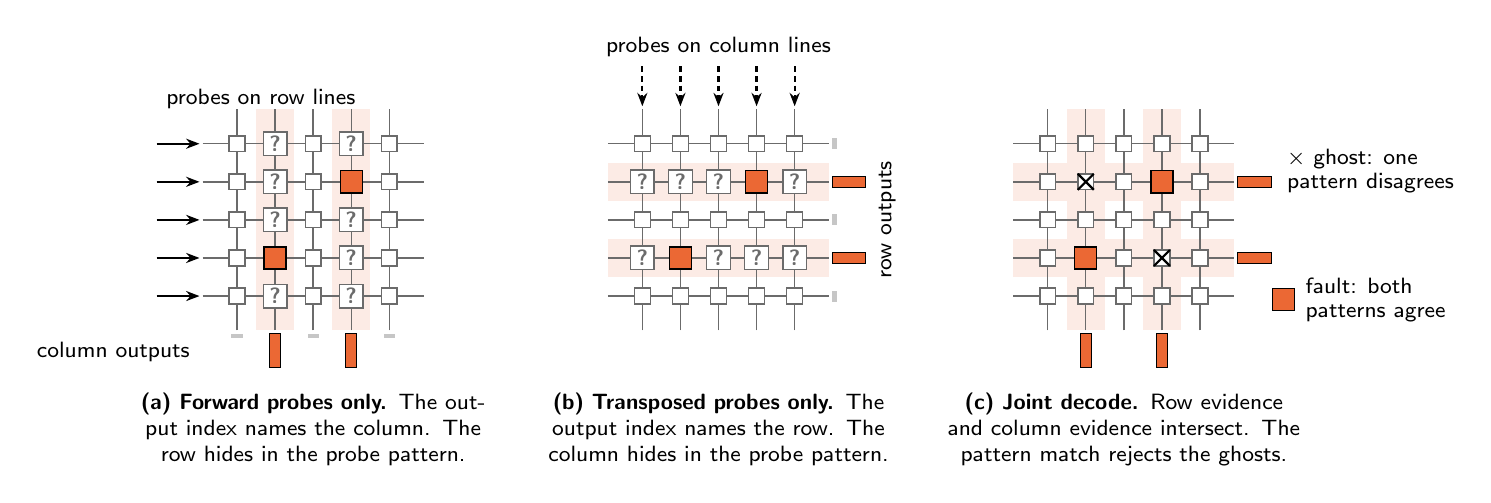
\begin{tikzpicture}[x=0.78cm,y=0.78cm]
%% ---------------- (a) forward only ----------------
\begin{scope}[shift={(0,0)}]
  \foreach \c in {2,4}{\fill[band] ({\X{\c}-0.31},-0.25) rectangle ({\X{\c}+0.31},3.35);}
  \grid \cells \faults
  \foreach \r in {1,2,3,5}{\node[unk] at ({\X{2}},{\Y{\r}}) {?};}
  \foreach \r in {1,3,4,5}{\node[unk] at ({\X{4}},{\Y{\r}}) {?};}
  \foreach \r in {1,...,5}{\draw[drv] (-1.0,{\Y{\r}}) -- (-0.3,{\Y{\r}});}
  \node[anchor=south west] at (-1.0,3.2) {probes on row lines};
  \foreach \c in {1,3,5}{\fill[quiet] ({\X{\c}-0.09},-0.3) rectangle ({\X{\c}+0.09},-0.38);}
  \foreach \c in {2,4}{\draw[flag] ({\X{\c}-0.09},-0.3) rectangle ({\X{\c}+0.09},-0.85);}
  \node[anchor=east] at (-0.3,-0.6) {column outputs};
  \node[anchor=north,align=center,text width=6.1cm] at (1.55,-1.1)
    {\textbf{(a) Forward probes only.} The output index names the column. The row hides in the probe pattern.};
\end{scope}
%% ---------------- (b) transposed only ----------------
\begin{scope}[shift={(6.6,0)}]
  \foreach \r in {2,4}{\fill[band] (-0.25,{\Y{\r}-0.31}) rectangle (3.35,{\Y{\r}+0.31});}
  \grid \cells \faults
  \foreach \c in {1,2,3,5}{\node[unk] at ({\X{\c}},{\Y{2}}) {?};}
  \foreach \c in {1,3,4,5}{\node[unk] at ({\X{\c}},{\Y{4}}) {?};}
  \foreach \c in {1,...,5}{\draw[drvb] ({\X{\c}},4.05) -- ({\X{\c}},3.4);}
  \node[anchor=south] at (1.55,4.05) {probes on column lines};
  \foreach \r in {1,3,5}{\fill[quiet] (3.4,{\Y{\r}-0.09}) rectangle (3.48,{\Y{\r}+0.09});}
  \foreach \r in {2,4}{\draw[flag] (3.4,{\Y{\r}-0.09}) rectangle (3.95,{\Y{\r}+0.09});}
  \node[rotate=90,anchor=north] at (4.0,1.55) {row outputs};
  \node[anchor=north,align=center,text width=6.1cm] at (1.55,-1.1)
    {\textbf{(b) Transposed probes only.} The output index names the row. The column hides in the probe pattern.};
\end{scope}
%% ---------------- (c) joint decode ----------------
\begin{scope}[shift={(13.2,0)}]
  \foreach \c in {2,4}{\fill[band] ({\X{\c}-0.31},-0.25) rectangle ({\X{\c}+0.31},3.35);}
  \foreach \r in {2,4}{\fill[band] (-0.25,{\Y{\r}-0.31}) rectangle (3.35,{\Y{\r}+0.31});}
  \grid \cells \faults
  \ghost{2}{2}\ghost{4}{4}
  \foreach \c in {2,4}{\draw[flag] ({\X{\c}-0.09},-0.3) rectangle ({\X{\c}+0.09},-0.85);}
  \foreach \r in {2,4}{\draw[flag] (3.4,{\Y{\r}-0.09}) rectangle (3.95,{\Y{\r}+0.09});}
  \node[anchor=west,align=left] at (4.05,2.35) {$\times$ ghost: one\\[-1pt]pattern disagrees};
  \node[bad] at (4.15,0.25) {};
  \node[anchor=west,align=left] at (4.35,0.25) {fault: both\\[-1pt]patterns agree};
  \node[anchor=north,align=center,text width=6.1cm] at (1.55,-1.1)
    {\textbf{(c) Joint decode.} Row evidence and column evidence intersect. The pattern match rejects the ghosts.};
\end{scope}
\end{tikzpicture}
\end{document}
